\section{Projetando o Polo Norte}


%%%%%%%%%%%%%%%%%%%%%%%%%%%%%%%%%%%%%%%%%%%%%%%%%%%%%%%%%%%%
\subsection{Introdução}

A projeção estereográfica é um mapeamento que projeta a 
esfera no plano, sendo definida em toda a esfera exceto 
em um ponto, neste caso escolheremos o 'polo norte'. Essa 
projeção é um funcional linear suave e bijetivo, é uma 
transformação conforme (preserva ângulos), mas não é uma 
isometria (não preserva distâncias nem áreas das figuras).

Seja a esfera $S_{\R}^2\subset\R^3 = \{(x,y,z)\in\R^3 \ 
| \ x^2 + y^2 + z^2 = R^2\}$, a projeção estereográfica é 
definida como o mapeamento no plano de um ponto $P(x,y,z)$
pertencente à esfera $S_{\R}^2$ em um ponto $P'(x',y')$ 
pertencente ao plano $\R^2$.

Em outras palavras projeta-se a esfera $S_{\R}^2$ através 
do 'polo norte' $N(0,0,R)$ no plano equatorial $z = 0$. 
A interseção de uma reta que liga o ponto $N$ e o plano
equatorial define um ponto $P'(x',y')$ no plano chamado 
de imagem estereográfica do ponto $P(x,y,z)$ definido 
pela interseção desta mesma reta com a esfera.


\begin{figure}[!h]
 \centering
 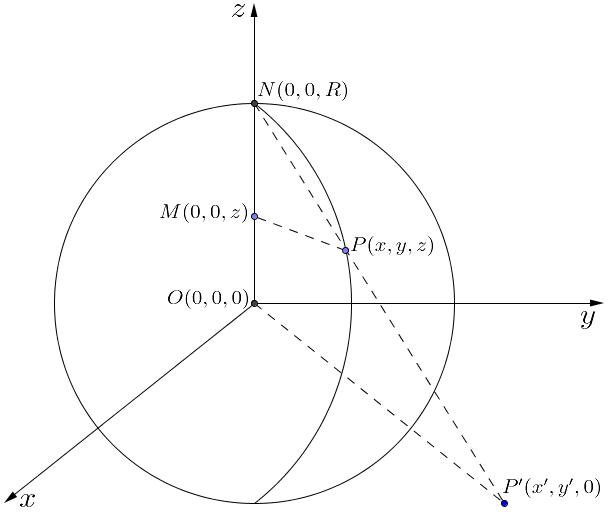
\includegraphics[scale=.6]{projecao1.JPG}
 \caption{Projeção Estereográfica da esfera no plano. 
 O ponto $P'(x',y')$ é a imagem
estereográfica do ponto $P(x,y,z)$.} 
\label{figura1}
\end{figure}



%%%%%%%%%%%%%%%%%%%%%%%%%%%%%%%%%%%%%%%%%%%%%%%%%%%%%%%%%%%%
\subsection{Coordenadas Cartesianas no Plano}

Analisando a figura anterior, temos dois triângulos 
retângulos semelhantes. Um deles é o triângulo $\Delta MNP$ 
e o outro é o triângulo $\Delta ONP'$:
%
\begin{equation}
\frac{\overline{MN}}{\overline{ON}} = 
\frac{\overline{MP}}{\overline{OP'}} 
\Rightarrow
\frac{z-R}{R} = \frac{\sqrt{x^2 + y^2}}
{\sqrt{{x'}^2 + {y'}^2}}
\end{equation}
%
Se fizermos $y = 0$ teremos também que $y' = 0$, pois 
movemos o ponto $P(x,y,z)$ para o plano $xOz$, mas os 
triângulos permanecem os mesmos. E se fizermos $x = 0$ 
teremos $x' = 0$ pois projetamos os triângulos para 
o plano $yOz$. Resolvendo individualmente as duas
condições encontramos que:
%
\begin{equation}
x' = \frac{Rx}{R - z} \qquad y' = \frac{Ry}{R - z}
\end{equation}
%
Elevando as duas relações encontradas para $x'$ e $y'$ 
ao quadrado temos que:
%
\begin{equation}
{x'}^2 + {y'}^2 = R^2\frac{(x^2 + y^2)}{(R-z)^2} 
= R^2\frac{(R^2 - z^2)}{(R-z)^2}
\end{equation}
%
Simplificando a relação acima temos que:
%
\[
{x'}^2 + {y'}^2  = R^2\frac{R + z}{R - z}
\]
%
Invertendo a transformação conforme, encontramos 
o seguinte resultado:
%
\[
\frac{z}{R} = \frac{{x'}^2 + {y'}^2 - R^2}
{{x'}^2 + {y'}^2 + R^2}
\]
%
Conhecendo este resultado podemos agora encontrar 
as relações para $x$ e $y$:
%
\begin{align}
x &= \left(1 - \frac{z}{R}\right)x' 
= \frac{2R^2x'}{{x'}^2 + {y'}^2 + R^2} 
\\
y &= \left(1 - \frac{z}{R}\right)y' 
= \frac{2R^2y'}{{x'}^2 + {y'}^2 + R^2}
\end{align}



%%%%%%%%%%%%%%%%%%%%%%%%%%%%%%%%%%%%%%%%%%%%%%%%%%%%%%%%%%%%
\subsection{Coordenadas Esféricas em Polares}

Agora iremos encontrar as coordenadas polares no 
plano $(\rho,\varphi')$ em função das coordenadas 
esféricas $(R,\theta,\varphi)$ e vice-versa. 
Utilizando a identidade $\rho = \sqrt{{x'}^2 + 
{y'}^2}$ e a relação para ${x'}^2 + {y'}^2$ deduzida 
anteriormente, temos que:
%
\[
{x'}^2 + {y'}^2 = \rho^2 = R^2
\frac{R + z}{R - z} \Rightarrow 
\rho = R\sqrt{\frac{R + z}{R - z}}
\]
%
Das coordenadas esféricas temos que $z = R\cos\theta$. 
Inserindo este resultado na equação anterior deduzida 
para $\rho$ chegamos ao seguinte resultado:
%
\[ 
\rho = \frac{R\sin\theta}{1 - \cos\theta}
\]
%
Lembrando das seguintes relações deduzidas na seção 
anterior:
%
\[ 
x' = \frac{Rx}{R - z} \qquad y' = \frac{Ry}{R - z}
\]
%
Podemos deduzir a relação para $\varphi$ em função das 
coordenadas esféricas:
%
\[
\tan\varphi' = \frac{y'}{x'} = \frac{y}{x} = 
\tan\varphi \Rightarrow \varphi' =
\varphi
\]
%
De modo que deduzimos as relações de transformação 
conforme entre as coordenadas esféricas e polares 
no plano.
%
\[
\left(\rho,\varphi'\right) 
\to \left(\frac{R\sin\theta}{1 - \cos\theta}, 
\varphi\right)
\]
%
Deduziremos agora as relações inversas $(R,\theta, 
\varphi)\to(\rho,\varphi)$. Temos que:
%
\[
\rho = \frac{R\sin\theta}{1 - \cos\theta} =
R\frac{2\sin(\theta/2)\cos(\theta/2)}
{2\sin^2(\theta/2)} = R\cot(\theta/2)
\]
%
Já foi mostrado que $\varphi' = \varphi$, então 
termina a demonstração da transformação inversa 
entre coordenadas esféricas e polares no plano:
%
\[
(\theta,\varphi) \to \left(\frac{1}{2} 
\cot^{-1}\left(\frac{\rho}{R}\right),\varphi'\right)
\]



%%%%%%%%%%%%%%%%%%%%%%%%%%%%%%%%%%%%%%%%%%%%%%%%%%%%%%%%%%%%
\subsection{Coordenadas Cilíndricas em Polares}

Nesta seção iremos encontrar a transformação de 
coordenadas cilíndricas $(r,\varphi,z)$ em coordenadas 
polares no plano $(\rho,\varphi')$. As coordenadas 
cilíndricas para as coordenadas dos pontos pertencentes 
à esfera são dadas por:
%
\begin{align}
r       &= \sqrt{x^2 + y^2}, 
\\
\varphi &= \tan^{-1}\left(\frac{y}{x}\right) 
\\
z'      &= z.
\end{align}
%
As coordenadas polares dos pontos pertencentes ao plano são:
%
\begin{align}
\rho     &= \sqrt{{x'}^2 + {y'}^2} 
\\ 
\varphi' &= \tan^{-1}\left(\frac{y}{x}\right).
\end{align}
%
Em coordenadas esféricas temos que $R = 
\sqrt{x^2 + y^2 + z^2}$. Comparando com as 
coordenadas cilíndricas:
%
\begin{equation}
(x, y, z) = (r\cos\varphi, r\sin\varphi, z), 
\end{equation}
%
tem-se que:
%
\begin{equation}
R^2 = r^2 + z^2 = \mbox{constante}.
\end{equation}
%
Em seções anteriores já foi demonstrado que:
%
\begin{equation}
x' = \frac{Rx}{R - z} \qquad , \qquad y' = \frac{Ry}{R - z}.
\end{equation}
%
De onde obtem-se imediatamente que:
%
\begin{equation}
\frac{y'}{x'} = \frac{y}{x} \Rightarrow \varphi = \varphi'.
\end{equation}
%
A seguinte relação também é imediata:
%
\begin{equation}
\rho^2 = {x'}^2 + {y'}^2 = \frac{R^2r^2}{(R - z)^2}, 
\end{equation}
%
que implica em:
%
\begin{equation}
\rho = \frac{Rr}{R -z}.
\end{equation}
%
Dessa maneira as relações de transformação das variáveis 
$(\rho,\varphi')$ nas variáveis $(r,\varphi,z)$ são 
as seguintes:
%
\begin{equation}
(\rho,\varphi') \to \left(\frac{Rr}{R - z},\varphi\right).
\end{equation}
%
Lembrando que $R(r,z) = \sqrt{r^2 + z^2}$ é uma função 
constante, dessa maneira é possível encontrar as relações 
inversas de transformação $(r,\varphi,z)\to(\rho,\varphi')$:
%
\begin{equation}
\rho = \frac{Rr}{R - z}, 
\end{equation}
%
implica que, 
%
\begin{equation}
z(\rho,\varphi') = \frac{\rho^2 - R^2}{\rho^2 + R^2}R.
\end{equation}
%
Utilizando-se do fato de que $r^2 = R^2 - z^2$ 
obtem-se que:
%
\begin{equation}
r(\rho,\varphi') = \frac{2R\rho}{\rho^2 + R^2}.
\end{equation}
%
Tem-se que as relações de transformação inversa são:
%
\begin{equation}
(r,\varphi,z) \to \left(\frac{2R\rho}{\rho^2 + R^2}, 
\varphi, \frac{\rho^2 - R^2}{\rho^2 + R^2}R\right).
\end{equation}
%


\begin{thebibliography}{}

\bibitem{Dubrovin}
Dubrovin, Fomenko, Novikov. Modern Geometry- Methods and Applications, 
Part 1, The Geometry of Surfaces, Transformation Groups and fields.

\end{thebibliography}